\chapter{一元多项式}
\section{一元多项式环}
\subsection{一元多项式的基本概念}
\emph{一元多项式并不是在中学便学习过了的一元多项式函数},两者有许多相似之处,但是前者的应用更加广泛。
在中学中,我们所学的 一元多项式函数$f(x)=a_nx^n+a_{n-1}x^{n-1}+\cdots+a_1x+a_0$并不需要其他额外的定义,其中 $x$便是
未知量,是一个待定的实数,和其他实数遵循同样的运算规律,从而整个函数也是这样,无需作特殊的定义。但是我们这里所学是:
\begin{mydef}[一元多项式]
   数域$K$上的一元多项式是指形如下述的表达式: 
\[a_nx^n+a_{n-1}x^{n-1}+\cdots+a_1x+a_0\]
\end{mydef}
1)它不是一个函数;2)其中的$x$被称为不定元,规定 $x^0=1$;3)它的系数 $a_{i}^{}$是 数域$K$中的一个元素,$a_0$称为零次项或常数项;
如果系数全为0,则称该多项式为零多项式,记作0,否则应有 $a_n\neq 0$。

第一点就意味着,在没有定义之前,”多项式1=多项式2“这样的等式是没有意义的。同时,把”多项式1=多项式2“中的
不定元$x$替换成一个实数来得到一个等式的操作也是需要证明才可以进行的。
\begin{myrmk}
    数域$K$上所有一元多项式的集合记作 $K[x]$。
\end{myrmk}
\begin{mydef}
    两个多项式相等的含义是系数非零的项完全相同。
\end{mydef}

第二点中的不定元是一个存粹的记号,不属于 数域$K$,因此实际上我们需要定义多项式的加法和乘法。
\begin{mydef}
    设 $f(x)=\sum_{t=0}^na_ix^i,g(x)=\sum_{t=0}^nb_ix^i,$不妨设 $m\leq n$,令
    \[f(x)+g(x):=\sum_{t=0}^n(a_i+b_i)x^i,\]
    \[f(x)g(x):=\sum_{s=0}^{m+n}(\sum_{i+j=s}^{}a_ib_j)x^s,\]
    \[-f(x):=\sum_{t=0}^n-a_ix^i,\]
    \[f(x)-g(x):=f(x)+[-g(x)].\]
\end{mydef}
\begin{myrmk}
    不定元$x$满足$x^ix^j=x^{i+j}$。

    既然不定元是一个记号,它可以用除了 $x$以外的其他符号来代替,常见的有 $\lambda$。
\end{myrmk}

和多项式函数一样,多项式 $f(x)=\sum_{t=0}^na_ix^i$也有”次数“的概念。 $a_ix_i$称为“$i$次项”( $i=1,2,\cdots,n$),
如果 $a_n\neq 0$,则称$a_nx^n$是 $f(x)$ 的首项,$n$是$f(x)$ 的次数,记作 $\deg f$。
\begin{myrmk}
    要注意区分零多项式0和零次多项式$a_0$($a_0\in K^*$)之间的区别。
\end{myrmk}
为了使得多项式 $f,g$ 的和与积的次数符合我们的直觉(尤其是当其中一个多项式为零多项式时),我们有规定零多项式的次数为 $-\infty$。
从而有
\begin{myprop}
    设 $f(x),g(x)\in K[x],$则
    \[\deg(f\pm g)\leq\max\{\deg f,\deg g\},\]
    \[\deg(f\cdot g)=\deg f+\deg g\]
\end{myprop}
\begin{myrmk}
    在证明与多项式相关的命题时,通常会依据其中的多项式是否有零多项式来展开分类讨论。
\end{myrmk}
\subsection{一元多项式环的性质}
至此,我们已经给出了有关多项式的基本定义。易知, $K[x]$构成一个整环。
\begin{mythm}[一元多项式环的通用性质]
    设 $K$是一个数域,$R$是一个有单位元 $1'$的交换环,它可以看成是 $K$的一个扩环,
    其中 $K$到 $R$的子环 $R_1$的保持加法和乘法运算的双射记作 $\tau$.任意给定 $t \in R$,令
    \[
    \begin{array}{rrcl}
    \sigma_{t} : &  K[x] & \longrightarrow  & \mathbf{R} \\
                   &  f(x)=\sum_{i=0}^{n}{a_ix^i}  & \longmapsto    & \sum_{i=0}^{n}{\tau(a_i)t^i}=:f(t), \\
    \end{array}
    \]
    则 $\sigma_t$是 $K[x]$到 $R$的一个映射,且它保持加法和乘法运算,即如果在 $K[x]$中,有
    \[f(x)+g(x)=h(x),\phantom{111}f(x)g(x)=p(x),\]
    那么在 $R$中,有
    \[f(t)+g(t)=h(t),\phantom{111}f(t)g(t)=p(t);\]
    还有 $\sigma_t(x)=t$。映射 $\sigma_t$称为 $x$用 $t$代入。
\end{mythm}

\begin{figure}
    \centering
    \caption{一元多项式环的通用性质}
    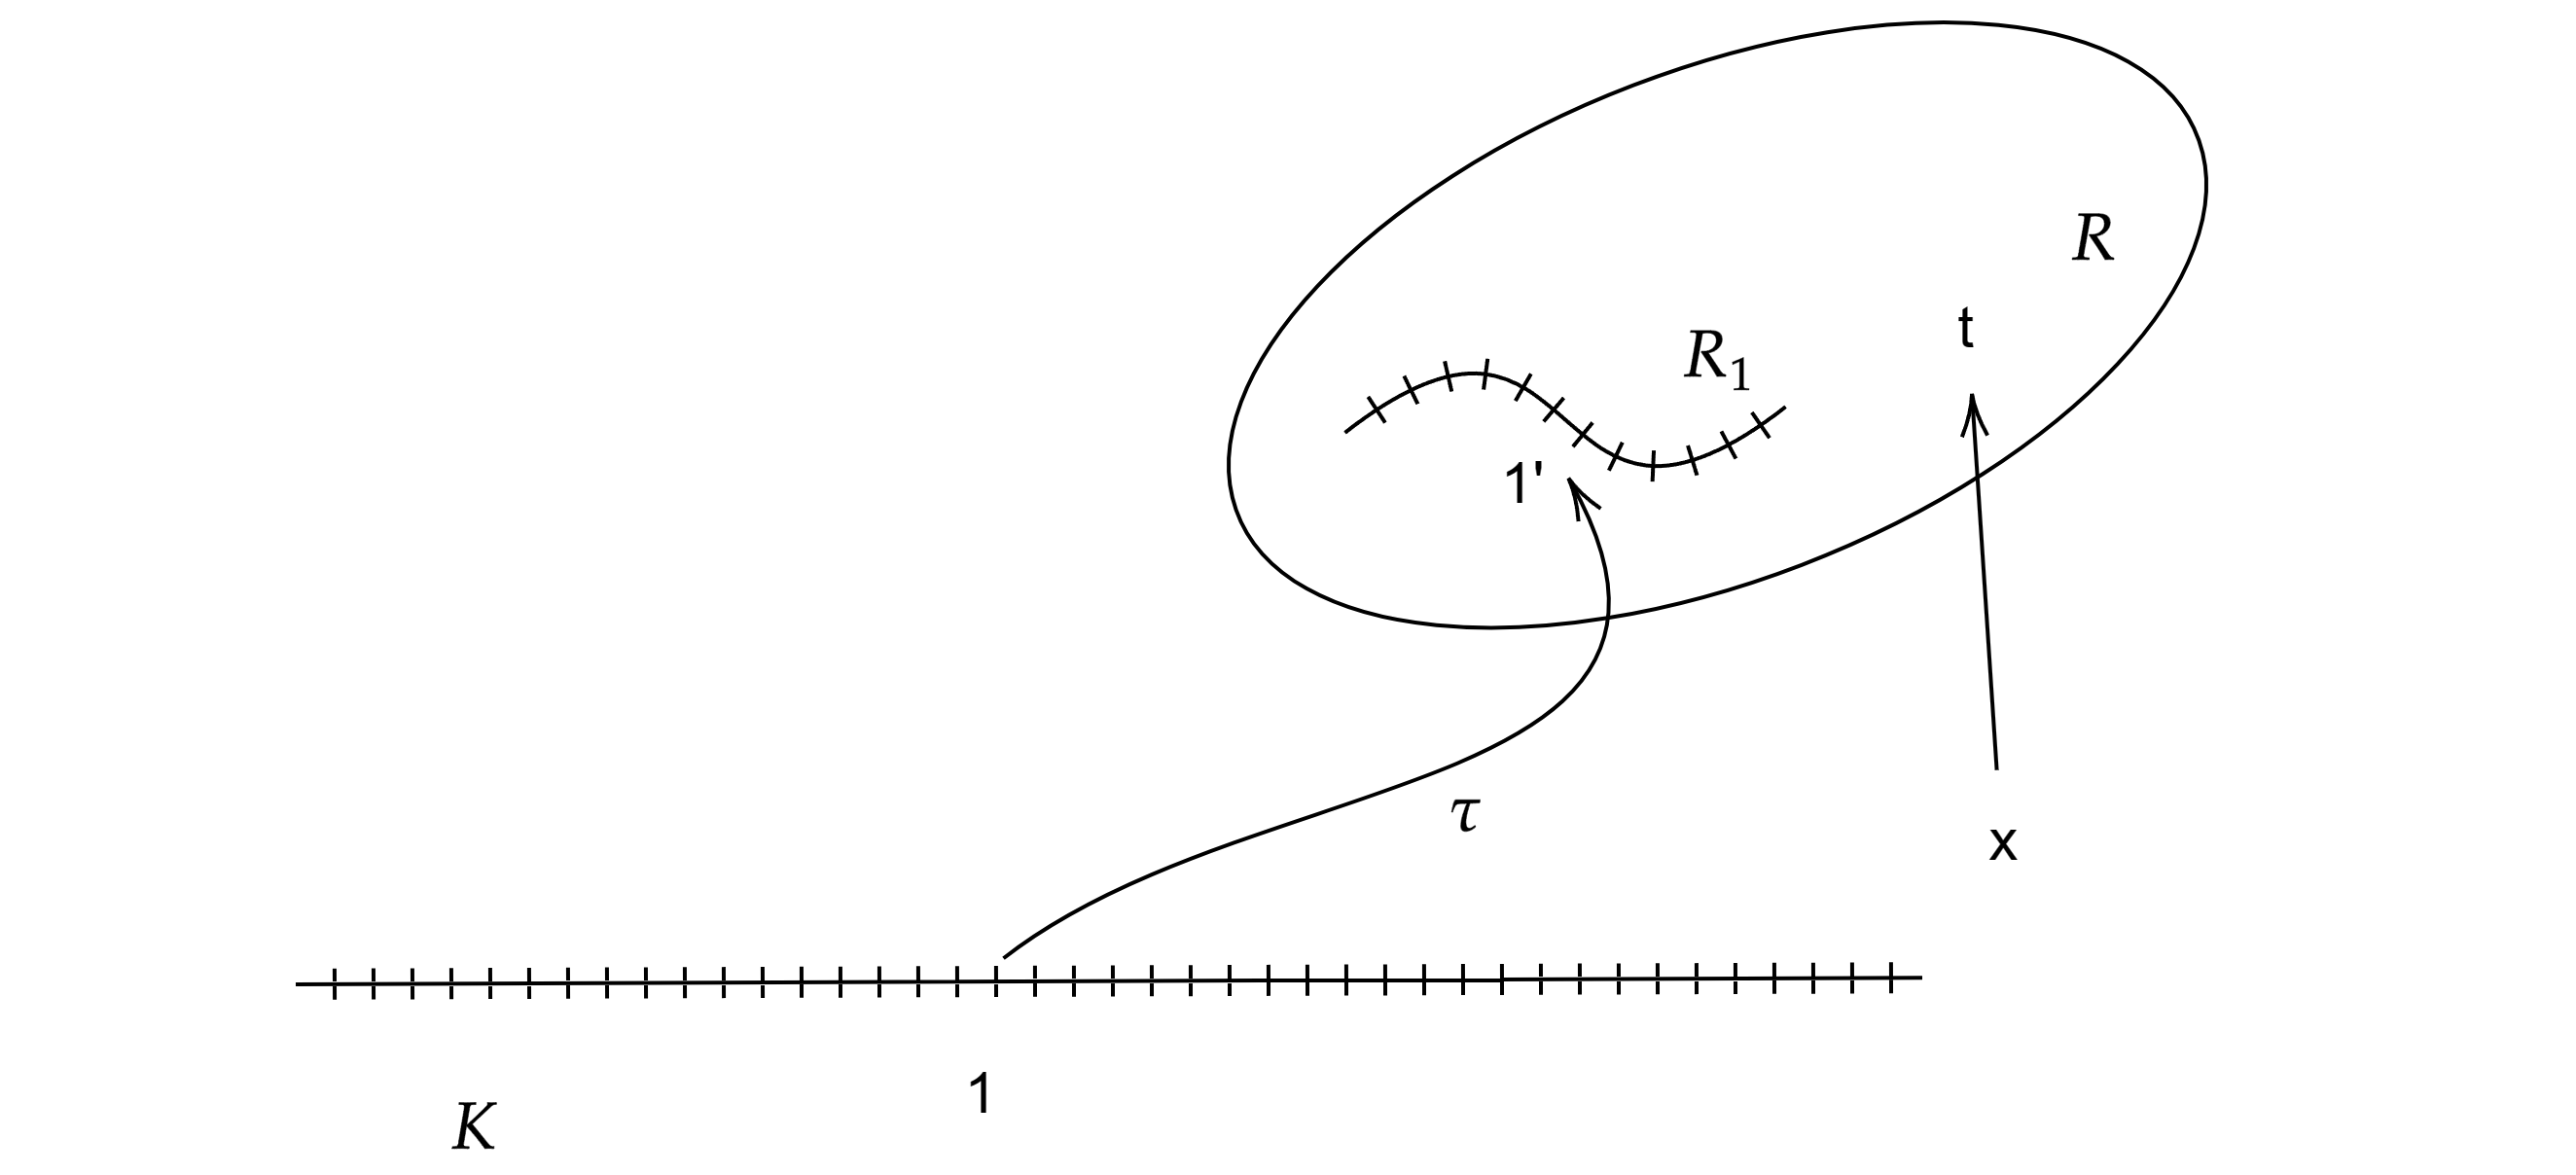
\includegraphics[width=\textwidth]{./pic/chapter1/扩环.png}
\end{figure}
\begin{myrmk}
    证明方法便是利用映射 $\sigma_t$以及加法和乘法的性质。

    从证明过程中可以看出,条件可以进一步放松:只要 $R$的元素 $t$与子环 $R_1$的元素可交换,那么 不定元$x$就可以用 $t$代入。

    同时,命题中的映射可以改变为
    \[
    \begin{array}{rrcl}
    \sigma_{t} : &  K[x^p] & \longrightarrow  & \mathbf{R} \\
                   &  f(x)=\sum_{i=0}^{n}{a_i(x^p)^i}  & \longmapsto    & \sum_{i=0}^{n}{\tau(a_i)t^i}=:f(t), \\
    \end{array}
    \]
    也就是说,这个命题可以拓展到关于 $x^p$的多项式。特别地,我们可以有 $\sigma_t(x^2)=a\in\mathbf{R^-}$,也就是说,虽然不定元有着”平方形式“,
    但是仍然可以代入数域中的一个非负元素。
\end{myrmk}
\begin{myrmk}
    常常对以下恒等式进行代换:
    \[
    \begin{array}{rcl}
        x^n-1&=&(x-1)(x^{n-1}+x^{n-2}+\cdots+x+1)\\
        x^n+1&=&(x+1)(x^{n-1}-x^{n-2}+\cdots+(-1)^{n-1-i}x+(-1)^{n-1})\\
        x^n-1&=&\prod_{i=0}^{n-1}(x-\omega^i)\\
    \end{array}    
    \]
    其中 $\omega$为 $n$次复单位根 $e^{i\frac{2\pi}{n}}$.
\end{myrmk}
这个定理允许我们将$K[x]$上关于加法和乘法的等式通过替换 不定元$x$来得到 数域$K$的扩环 $R$上的等式。
常常利用这个性质来得到 $K[x],K,M_n(K)$上的等式(例如将 不定元$x$分别替换为 $cx$,$c$,$A$,对应扩环关系中的子环是由 $a,a,a\mathbf{I},a\in K$组成,
其中第一个 $a$是零次多项式或零多项式 )
\section{整除关系与带余除法}
\subsection{整除关系}
\begin{mydef}[整除]
    设 $f(x),g(x)\in K[x]$,如果存在 $h(x)\in K[x],$使得 $f(x)=h(x)g(x),$那么
    称 $g(x)$整除 $f(x)$,记作 $g(x)\mid f(x)$;否则,称 $g(x)$不能整除 $f(x)$,记作 $g(x)\nmid f(x)$。
\end{mydef}
    当 $g(x)$整除 $f(x)$时,称 $g(x)$是 $f(x)$的一个因式,称 $f(x)$是 $g(x)$的一个倍式。
\begin{myrmk}
    判断 $g$能否整除 $f$,实际上就是要判断能否找到一个因子 $h$,使得 $f=h\cdot g$。新增的因子按照惯例应该写在 $g$之前。
\end{myrmk}
由整除定义可以得到以下性质:
\begin{myproperty}
\begin{enumerate}
\item $0\mid f(x)\phantom{11}\Longleftrightarrow\phantom{11}f(x)=0$;
\item $f(x)\mid 0,\forall f(x)\in K[x];$
\item $b\mid f(x),\forall b\in K^*,\forall f(x)\in K[x].$
\end{enumerate}
\end{myproperty}
\begin{myrmk}
    整除关系实际上是通过乘法来定义的,因此整除0是合法的。
\end{myrmk}
\begin{myrmk}
    整除是集合 $K[x]$中的一个二元关系,它具有反身性和传递性,但是不具有对称性。
\end{myrmk}
\begin{mydef}[相伴]
    在 $K[x]$中,如果 $g(x)\mid f(x)$且 $f(x)\mid g(x)$,那么称 $f(x)$与 $g(x)$相伴,记作 $f(x)\sim g(x)$。
\end{mydef}
\begin{myprop}
    在 $K[x]$中,$f(x)\sim g(x)$当且仅当存在 $c\in K^*$,使得
    \[f(x)=cg(x).\]
\end{myprop}
\begin{myprop}
    在 $K[x]$中,如果 $g(x)\mid f_i(x),i=1,2,\cdots,s$,那么对于任意 $u_1(x),\cdots,u_s(x)\in K[x]$,
    都有 
    \[g(x)\mid [u_1(x)f_1(x)+\cdots+u_s(x)f_s(x)].\]
\end{myprop}
\subsection{带余除法}
\begin{mythm}[带余除法]
    设 $f(x),g(x)\in K[x],$且 $g(x)\neq 0.$则在 $K[x]$中存在唯一的一对多项式 $h(x),r(x)$,
    使得
    \[f(x)=h(x)g(x)+r(x),\phantom{111}\deg r(x)<\deg g(x),\]
    其中 $f(x)$,$g(x)$分别叫做被除式,除式,$h(x),r(x)$分别叫做商式,余式。上式称为除法算式。
\end{mythm}
\begin{myrmk}
    显然,除法算式中的余式为零多项式当且仅当 $g\mid f$。
\end{myrmk}
\begin{myprop}
    设 $f(x),g(x)\in K[x],$数域 $F\supseteq K,$则在 $K[x]$中, $g(x)\mid f(x)\Leftrightarrow$
    在 $F[x]$中 ,$g(x)\mid f(x)$.
\end{myprop}
\begin{myrmk}
    此即整除性不随数域的扩大而改变.
\end{myrmk}
\section{最大公因式}
\subsection{基本概念}
\begin{mydef}[公因式]
  在 $K[x]$中,若 $c(x)\mid f(x)$且 $c(x)\mid g(x)$,则称 $c(x)$是 $f(x)$与 $g(x)$的一个公因式。  
\end{mydef}
\begin{mydef}[最大公因式]
    $K[x]$中多项式 $f(x)$与 $g(x)$的一个公因式 $d(x)$如果满足下述条件:对于 $f(x)$
    与 $g(x)$的任一公因式 $c(x)$,都有 $c(x)\mid d(x)$,那么称 $d(x)$是 $f(x)$与 $g(x)$的一个最大公因式.
\end{mydef}
易知, $f(x)$与0的最大公因式是0.如果 $f(x)$与 $g(x)$不全为零多项式,则它们的最大公因式也不是零多项式。

在相伴意义下,若存在,则$f(x)$与 $g(x)$的最大公因式是唯一的。特别地,我们用 $(f(x),g(x))$来表示首项系数为1的最大公因式,称为 $f(x)$与 $g(x)$的
首一最大公因式。
\begin{mylmm}
    设 $f(x),g(x)\in K[x],$如果在 $K[x]$中有下述等式成立:
    \[f(x)=h(x)g(x)+r(x),\]
    那么\quad $c(x)\mid f(x)$且 $c(x)\mid g(x)\Leftrightarrow c(x)\mid g(x)$且 $c(x)\mid r(x);$

    从而, $d(x)$是 $f(x)$ 与 $g(x)$的最大公因式当且仅当 $d(x)$是 $g(x)$与 $r(x)$ 的最大公因式。
\end{mylmm}
\begin{myrmk}
    该引理的意义在于将除式与被除式的最大公因式转化为除式与余式的最大公因式,这便是辗转相除法的依据。
\end{myrmk}
\begin{mythm}
    对于 $K[x]$中任意两个多项式 $f(x)$与 $g(x)$,存在它们的一个最大公因式 $d(x)$,
    并且存在 $u(x),v(x)\in K[x]$,使得
    \[d(x)=u(x)f(x)+v(x)g(x).\]
\end{mythm}
\begin{myrmk}
该定理的证明中运用了辗转相除法.
\end{myrmk}
在求解最大公因式时,可以用下述命题降低复杂度:
\begin{myprop}
    设 $f(x),g(x)\in K[x],a,b\in K^*$,则 $d(x)$是 $f(x)$ 与 $g(x)$的最大公因式当且仅当 $d(x)$ 是 $af(x)$与 $bg(x)$的一个最大公因式。
\end{myprop}
\begin{myprop}
    $K[x]$中,设 $d(x)$是 $f(x)$与 $g(x)$的一个最大公因式,则对任意 $a\in K^*$都有 $ad(x)$是 $f(x)$与 $g(x)$的最大公因式。
\end{myprop}
\begin{myprop}
    设 $f(x)$ 与 $g(x)\in K[x]$,数域$F\supseteq K$,则 $f(x)$与 $g(x)$在 $K[x]$中
    的首一最大公因式等于它们在 $F[x]$中的首一最大公因式.即 $f(x)$与 $g(x)$的首一最大公因式
    不随数域的扩大而改变.
\end{myprop}
\begin{myprop}
    设 $f(x),g(x)\in K[x],$ 且 $f(x)$与 $g(x)$全不为0;设 $a,b,c,d\in K$,使得 $ad-bc\neq 0$。则 
    \[(af(x)+bg(x),cf(x)+dg(x))=(f(x),g(x)).\]
\end{myprop}
\begin{myrmk}
    该命题说明两个多项式经过可逆线性组合后,最大公因式保持不变。
\end{myrmk}
\subsection{互素公因式}
\begin{mydef}
    设 $f(x)$,$g(x)\in K[x]$,如果 $(f(x),g(x))=1$,那么称 $f(x)$与 $g(x)$互素.
\end{mydef}
\begin{myrmk}
    也就是说,此时两个公因式的最大公因式组成的集合便是 $K^*$。
\end{myrmk}
\begin{mythm}
    $K[x]$中 两个多项式 $f(x)$与 $g(x)$互素的充分必要条件是,存在 $u(x),v(x)\in K[x],$使得
    \[u(x)f(x)+v(x)g(x)=1.\]
\end{mythm}
\begin{myrmk}
    这个关于互素的定理是一个充要条件,而之前由辗转相除法得到的定理是单向的。
\end{myrmk}
\begin{mycor}
    设 $f(x),g(x)\in K[x]$,数域 $F\supseteq K$,则 $f(x)$与 $g(x)$在 $K[x]$中
    互素当且仅当 $f(x)$与 $g(x)$在 $F[x]$中互素.即互素性不随数域的扩大而改变。
\end{mycor}
\begin{myproperty}
    在 $K[x]$中,
\begin{enumerate}
\item 如果 $f(x)\mid g(x)h(x),$且 $(f(x),g(x))=1$,那么 $f(x)\mid h(x).$
\item 如果 $f(x)\mid h(x),g(x)\mid h(x),$且 $(f(x),g(x))=1$,那么 $f(x)g(x)\mid h(x)$.
\item 如果 $(f(x),h(x))=1,(g(x),h(x))=1$,那么 $(f(x)g(x),h(x))=1.$
\item 如果 $(f_i(x),h(x))=1,i=1,2,\cdots,s$,那么 $(f_1(x)f_2(x)\cdots f_s(x),h(x))=1.$
\end{enumerate}
\end{myproperty}
\begin{myrmk}
    为了方便直观地理解上述性质,可以将互素理解为“相互之间不包含组成对方的因子”,将整除理解为“包含组成对方的因子”,将相乘理解为“因子叠加”。
\end{myrmk}
\begin{myprop}
    在 $K[x]$中,如果 $(f,g)=1$,那么:
    \begin{enumerate}
        \item $(f,f+g)=(g,f+g)=1$
        \item $(fg,f+g)=1$
    \end{enumerate}
\end{myprop}
\begin{myrmk}
    第一条的证明利用了可逆线性变换时,最大公因式不变的性质。第二条利用了互素多项式的性质3.
\end{myrmk}
\begin{myprop}
    设 $A\in M_n(K),f(x),g(x)\in K[x]$,则如果 $d(x)$是 $f(x)$ 与 $g(x)$的一个最大公因式,那么齐次方程组 $d(A)x=0$的解空间 $W_3$等于 $f(A)x=0$
    的解空间 $W_1$与 $g(A)x=0$的解空间 $W_2$的交。
\end{myprop}
\begin{myprop}
    设 $A\in M_n(K),f_1(x),f_2(x)\in K[x]$,记 $f(x)=f_1(x)f_2(x)$。则如果 $(f_1(x),f_2(x))=1$,那么 $f(A)x=0$的任一个解可以唯一地表示
    成 $f_1(A)x=0$的一个解与 $f_2(A)x=0$的一个解的和。
\end{myprop}
\begin{myprop}
    设 $m,n\in N*$,则在 $K[x]$中,
    \[(x^m-1,x^n-1)=x^{(m,n)}-1.\]
\end{myprop}
\begin{myrmk}
    结合等式 $(m,n)=(n,m-n)$利用数学归纳法证明。
\end{myrmk}
\subsection{多个多项式的最大公因式和互素的多项式}
\begin{mydef}
    $K[x]$中,$f_1(x),f_2(x),\cdots,f_s(x)$的一个公因式 $d(x)$如果满足下述条件:
    $f_1(x),f_2(x),\cdots,f_s(x)$的任一公因式 $c(x)$都能整除 $d(x)$,那么称 $d(x)$为 
    $f_1(x),f_2(x),\cdots,f_s(x)$的一个最大公因式.
\end{mydef}
如果 $f_i(x)$不全为零多项式,则它们的最大公因式也不是零多项式。

在相伴意义下,若存在,则$f_1(x),\cdots,f_s(x)$的最大公因式是唯一的。特别地,我们用 $(f_1(x),\cdots,f_s(x))$来表示首项系数为1的最大公因式,称为
首一最大公因式。
\begin{mythm}
    在 $K[x]$中,对于 $s$个不全为0的多项式 $f_1(x),f_2(x),\cdots,f_s(x),$有多项式 $u_i(x),i=1,2,\cdots,s,$
    使得
    \[u_1(x)f_1(x)+\cdots + u_s(x)f_s(x)=(f_1(x),\cdots,f_s(x)).\]
\end{mythm}
\begin{mydef}
    在 $K[x]$中, $s$个多项式 $f_1(x),f_2(x),\cdots,f_s(x)$如果满足 $(f_1(x),f_2(x),\cdots,f_s(x))=1,$
    那么称 $f_1(x),f_2(x),\cdots,f_s(x)$互素.
\end{mydef}
\begin{mythm}
    在 $K[x]$中, $f_1(x),f_2(x),\cdots,f_s(x)$互素的充分必要条件是,存在 $u_1(x),u_2(x),\cdots,u_s(x)\in K[x],$
    使得 
    \[u_1(x)f_1(x)+\cdots+u_s(x)f_s(x)=1.\]
\end{mythm}
\begin{myrmk}
    当三个或三个以上的多项式互素时,它们不一定两两互素。因为前者表示它们没有共同的度数为正的因子,但是并不代表两两之间不存在。
\end{myrmk}
\section{最小公倍式}
\begin{mydef}
  设 $f(x),g(x)\in K[x],K[x]$中一个多项式 $m(x)$称为 $f(x)$ 与  $g(x)$的最小公倍式,如果 
  \begin{enumerate}
    \item $f(x)\mid m(x),g(x)\mid m(x);$
    \item $f(x)\mid u(x),g(x)\mid u(x)\Rightarrow m(x)\mid u(x).$
  \end{enumerate}  
\end{mydef}
\begin{myprop}
    在 $K[x]$中,任意两个多项式都有最小公倍式,并且 $f(x)$与 $g(x)$的最小公倍式在相伴意义下是唯一的。
\end{myprop}
我们用 $[f(x),g(x)]$来表示首项系数为1的最小公倍式。
\begin{myprop}
    如果 $f(x)$与 $g(x)$的首项系数为1,则
    \[[f(x),g(x)]=\frac{f(x)g(x)}{(f(x),g(x))}.\]
\end{myprop}

\section{不可约多项式与唯一因式分解定理}
\begin{mydef}
    设 $f(x)$是 $K[x]$中一个\emph{次数大于0}的多项式,如果 $f(x)$在 $K[x]$中的因式只有零次多项式,
    和 $f(x)$的相伴元,那么称 $f(x)$是 数域$K$上的一个不可约多项式;否则称 $f(x)$在 $K$上是可约的。
\end{mydef}
\begin{mythm}
    设 $p(x)$是 $K[x]$中一个次数大于0的多项式,则下列命题等价:
    \begin{enumerate}
        \item $p(x)$是不可约多项式;
        \item $\forall f(x)\in K[x]$,有 $p(x)\mid f(x)$或 $(p(x),f(x))=1$;
        \item 在 $K[x]$中,从 $p(x)\mid f(x)g(x)$可推出 $p(x)\mid f(x)$或 $p(x)\mid g(x)$;
        \item 在 $K[x]$中, $p(x)$不能被分解成两个次数较低的多项式的乘积。
    \end{enumerate}
\end{mythm}
\begin{myrmk}
    从而可以推出 $K[x]$中次数大于0的多项式 $f(x)$可约当且仅当 $f(x)$可以分解成两个次数较低的多项式的乘积。
\end{myrmk}
\begin{myrmk}
    也可以推出:只要 $g(x)$是 $K$上不可约多项式,就有:
    \[g(x)\mid f^m(x)\Leftrightarrow g(x)\mid f(x).\]
\end{myrmk}
\begin{mythm}[唯一因式分解定理]
   $K[x]$中任一次数大于0的多项式 $f(x)$能够唯一地分解成 数域$K$上有限多个不可约多项式的乘积。所谓唯一性是指,如果 $f(x)$有两个这样的分解式:
   \[f(x)=p_1(x)p_2(x)\cdots p_s(x)=q_1(x)q_2(x)\cdots q_t(x),\]
   那么一定有 $s=t$,且适当排列因式次序后有
   \[p_i(x)\sim q_i(x),\quad i=1,2,\cdots,s.\] 
\end{mythm}
$K[x]$中次数大于0的多项式 $f(x)$的标准分解式为:
\[f(x)=ap_1^{l_1}(x)p_2^{l_2}(x)\cdots p_s^{l_s}(x),\]
其中 $a$为 $f(x)$的首项系数; $p_1(x),p_2(x),\cdots,p_s(x)$是 $K$上两两不等的首一不可约多项式; $l_i>0,i=1,2,\cdots,s$。
如果知道 $K[x]$中的两个次数大于0的多项式 $f(x),g(x)$的标准分解式:
\[f(x)=ap_1^{l_1}(x)p_2^{l_2}(x)\cdots p_s^{l_s}(x),\]
\[g(x)=bp_1^{r_1}(x)p_2^{r_2}(x)\cdots p_m^{l_m}(x)q_1^{t_1}(x)\cdots q_n^{t_n}(x),(m\leq s),\]
那么
\[(f(x),g(x))=p_1^{\min\{l_1,r_1\}}(x)\cdots p_m^{\min\{l_m,r_m\}}(x);\]
\[[f(x),g(x)]=p_1^{\max\{l_1,r_1\}}(x)\cdots p_m^{\max\{l_m,r_m\}}(x)p_{m+1}^{l_{m+1}}(x)\cdots p_s^{l_s}(x)q_1^{t_1}(x)\cdots q_n^{t_n}(x);\]
\section{重因式}
当 $g(x)$整除 $f(x)$时,称 $g(x)$是 $f(x)$的一个因式,称 $f(x)$是 $g(x)$的一个倍式。 
\begin{mydef}[重因式]
    $K[x]$中,不可约多项式 $p(x)$称为 $f(x)$的 $k$重因式,如果 $p^k(x)\mid f(x)$,而 $p^{k+1}(x)\nmid f(x)$。
    
    如果 $k=0$,那么称 $p(x)$不是 $f(x)$的因式;如果 $k=1$,那么称 $p(x)$是 $f(x)$的单因式;如果 $k>1$,那么称 $p(x)$是 $f(x)$的重因式。
\end{mydef}
\begin{mydef}
    对于 $K[x]$中的多项式 
    \[f(x)=a_nx^n+a_{n-1}x^{n-1}+\cdots+a_1x+a_0,\]
    我们把多项式 
    \[na_nx^{n-1}+(n-1)a_{n-1}x^{n-2}+\cdots+a_1\]
    称为 $f(x)$的导数(或一阶导数),记作 $f^{\prime}(x)$。
\end{mydef}
\begin{mythm}
    设 $K$是数域,在 $K[x]$中,如果不可约多项式  $p(x)$是 $f(x)$的一个 $k(k\geq 1)$重因式,那么 $p(x)$是 $f^{\prime}(x)$的一个 $k-1$
    重因式。特别地, $f(x)$的单因式不是 $f^{\prime}(x)$的因式。
\end{mythm}
\begin{mycor}
    设 $K$是数域,在 $K[x]$中,不可约多项式  $p(x)$是 $f(x)$的一个重因式,当且仅当 $p(x)$是 $f(x)$与 $f^{\prime}(x)$的一个公因式。
\end{mycor}
\begin{mycor}
    设 $K$是数域,在 $K[x]$中,不可约多项式  次数大于0$f(x)$有重因式,当且仅当 $f(x)$与 $f^{\prime}(x)$有次数大于0的公因式。
\end{mycor}
\begin{mycor}
    设 $K$是数域,在 $K[x]$中,不可约多项式  次数大于0$f(x)$没有重因式,当且仅当 $f(x)$与 $f^{\prime}(x)$互素。
\end{mycor}
\begin{mycor}
    设 数域$F$包含 数域$K$,对于 $K[x]$中次数大于0的多项式 $f(x)$, $f(x)$在 $K[x]$中没有重因式当且仅当 $f(x)$在 $F[x]$中没有重因式,即 $f(x)$
    有无重因式不会随数域的扩大而改变。
\end{mycor}
想要获取和 $f(x)$含有完全相同的不可约因式(不计重数),但又不含重因式的多项式 $g(x)$,我们有:
\[g(x)=\frac{f(x)}{(f(x),f^{\prime}(x))}\]
\section{整数环 $\mathbf{Z}$中的定理与性质}
在整数环 $\mathbf{Z}$中,也有一系列对应的关于整除的定理和性质:
\begin{mythm}
    任给 $a,b\in \mathbf{Z},b\neq 0,$则存在唯一的一对整数 $q,r$,使得
    \[a=qb+r,\phantom{1111}0\leq r<\abs{b}.\]
\end{mythm}